\chapter{Gráficas}

\section{Gráficas en dos dimensiones}

MATLAB dispone de una gran variedad de funciones y herramientas que permiten crear gráficas de casi 
cualquier tipo, tanto en dos dimensiones como superficies y curvas tridimensionales. Además, MATLAB 
proporciona una facilidad extraordinaria para personalizar las gráficas mediante la inclusión de 
anotaciones, etiquetas, mapas de colores y muchos otros elementos que permiten una mayor legibilidad 
e interactividad con la información presentada en los gráficos. En este capítulo se tratarán las 
gráficas en dos dimensiones, en el espacio y además, una introducción a las animaciones.

\subsection{Una introducción: la función plot}

La función plot es una instrucción muy sencilla que permite trazar curvas bidimensionales utilizando 
vectores como argumentos. Por ejemplo si necesita graficar la función seno en el intervalo de $-\pi$ a $\pi$, 
necesita crear primeramente un vector con un determinado número de elementos para definir el dominio a 
graficar y enseguida aplicar a ese vector la función matemática que corresponda. Para crear un vector que 
defina el dominio puede hacerlo de diversas formas (revise la sección 2.1). A continuación se especifican 
las líneas de código necesario para crear la gráfica antes mencionada y el resultado de salida:

\begin{verbatim}
	x=-pi:pi/180:pi;
	y=sin(x);
	plot(x,y);
\end{verbatim}

\begin{center}
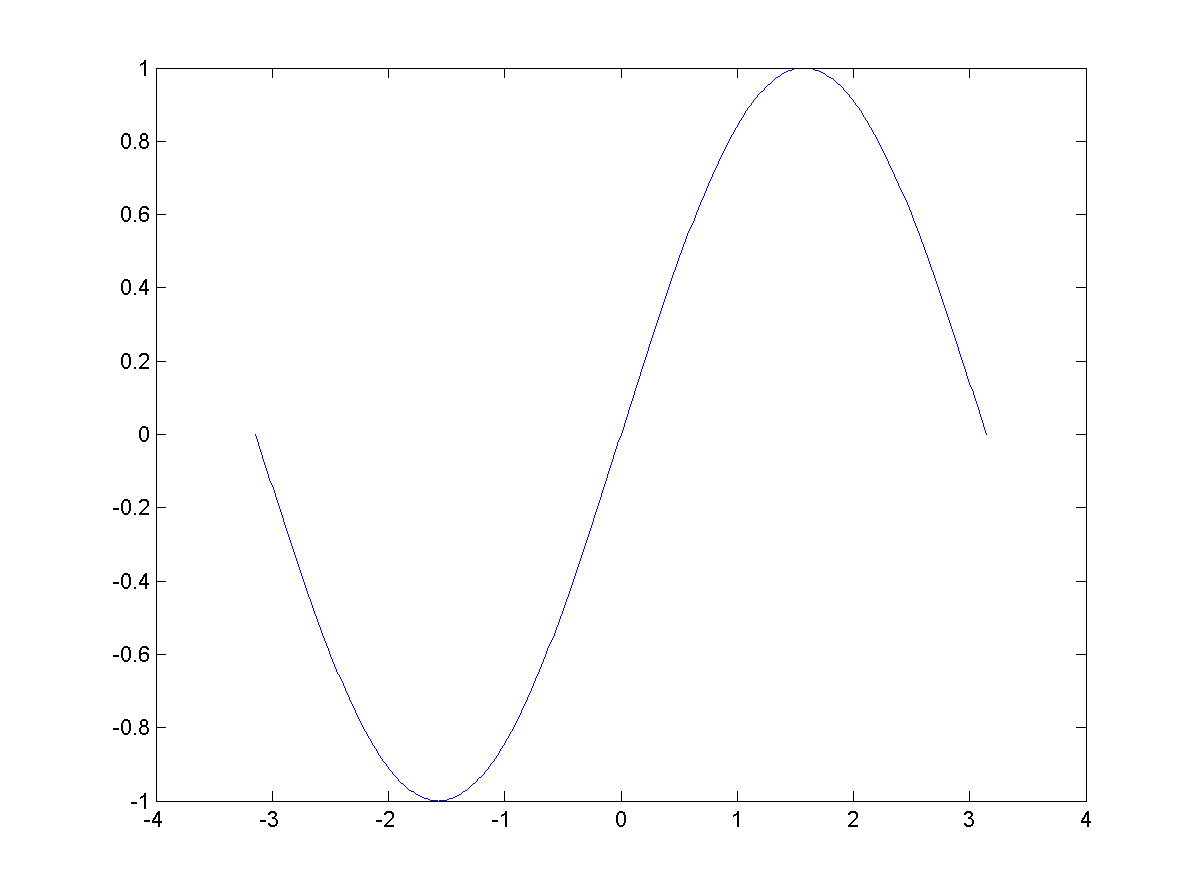
\includegraphics[scale=0.6]{src/ch4/img_4_1.png}
\captionof{figure}{Gráfica en 2D en coordenadas rectangulares}
\end{center}

\subsubsection{Graficar más de una función}

Si necesita incluir dos o más gráficas en una misma ventana puede utilizar el comando 
hold on para permitir que MATLAB simplemente agregue las gráficas sin borrar las ya 
existentes, por ejemplo:

\begin{verbatim}
	x=-pi:pi/180:pi;
	y1=sin(x);
	y2=cos(x);
	y3=cos(x+pi/3);
	hold on
	plot(x,y1);
	plot(x,y2);
	plot(x,y3);
\end{verbatim}

\begin{center}
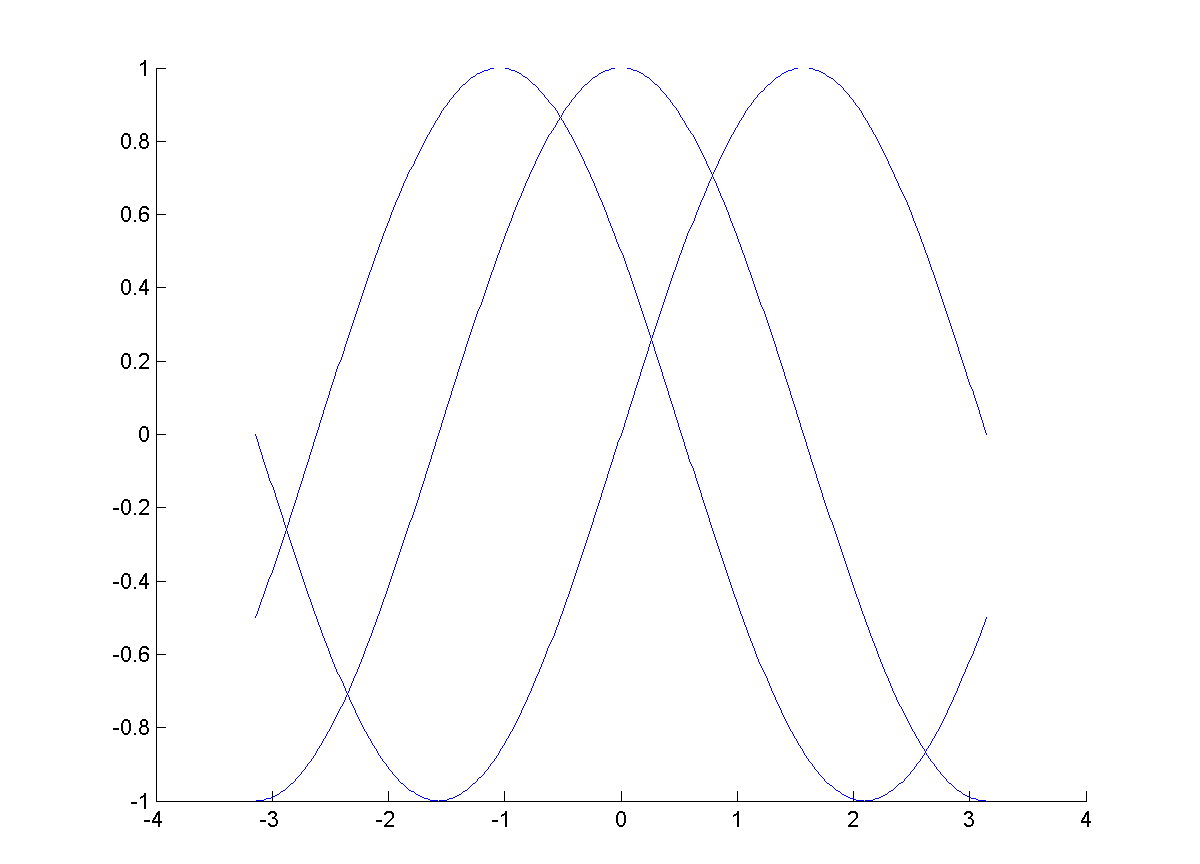
\includegraphics[scale=0.6]{src/ch4/img_4_2.png}
\captionof{figure}{Dos gráficas en una misma ventana}
\end{center}

Lo anterior funciona incluso para cuando se tienen intervalos diferentes. Si necesita 
graficar dos o más funciones en un mismo intervalo, es decir utilizando el mismo vector 
como variable independiente, puede utilizar la siguiente forma más compacta para agregar 
más de una función sin recurrir al comando descrito con anterioridad:

\begin{verbatim}
	x=-pi:pi/180:pi;
	y1=sin(x);
	y2=cos(x);
	y3=cos(x+pi/3);
	plot(x,[y1;y2;y3]);
\end{verbatim}

\begin{center}
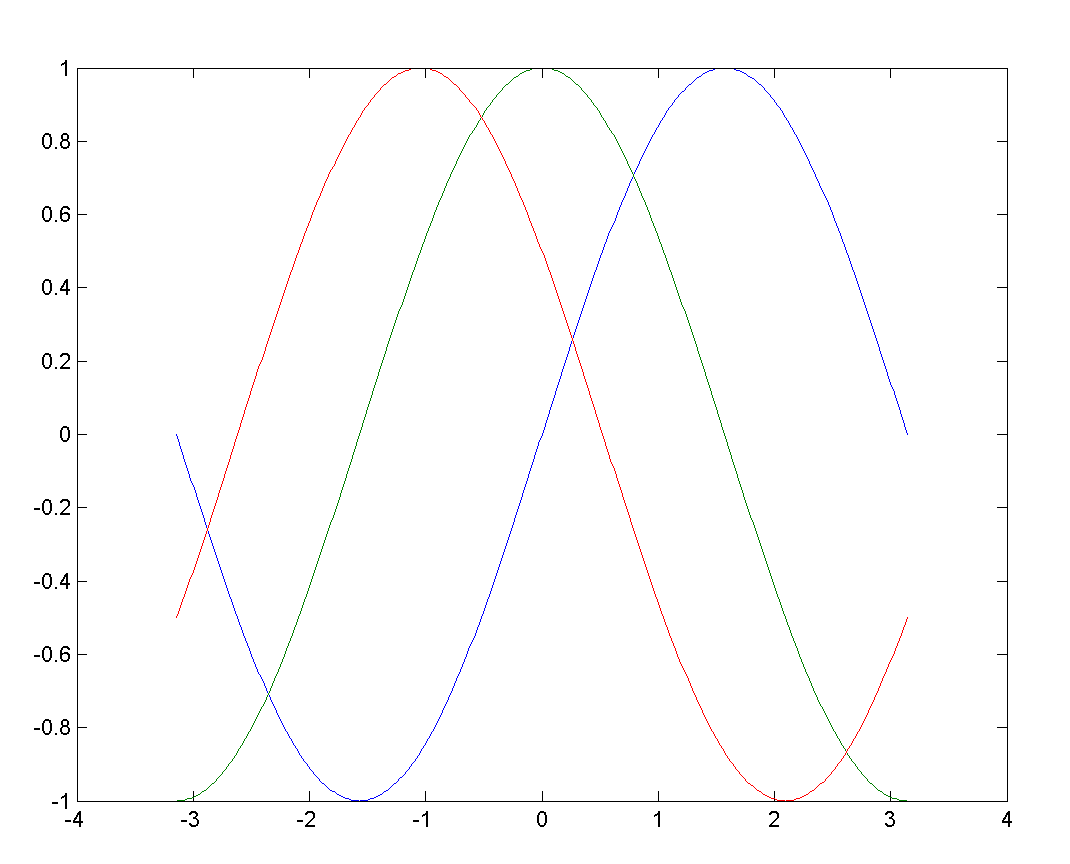
\includegraphics[scale=0.6]{src/ch4/img_4_3.png}
\captionof{figure}{Dos gráficas en una misma ventana}
\end{center}

En lugar de utilizar hold on puede configurar la propiedad NextPlot del axes de tal manera 
que las gráficas sean agregadas sin borrar los objetos que pertenecen al axes. Lo anterior 
se logra con la siguiente línea de código:

\begin{verbatim}
	set(gca,'NextPlot','add');
\end{verbatim}

Quizá lo anterior resulte un poco avanzado para comenzar, pero puede tomarse simplemente 
como una observación muy útil de que en MATLAB pueden implementarse diversas soluciones a 
un mismo problema o requerimiento.

\subsection{Configurar propiedades de las gráficas}

\subsubsection{Añadir etiquetas, leyendas y títulos}

En la sección anterior se han visto los pasos para mínimos para trazar una gráfica, pero 
ésta todavía puede resultar poco útil dado que no contiene información de ningún tipo 
acerca de los datos graficados. Es posible añadir etiquetas a los ejes con las funciones 
xlabel, ylabel y zlabel, además de poder añadir una identificación de una determinada 
curva mediante la función \texttt{legend} e incluso colocar un título en la parte superior con la 
función \texttt{title}:

\begin{verbatim}
	x=-pi:pi/180:pi;
	y=sin(x);
	plot(x,y);
	xlabel('Eje X');
	ylabel('Eje Y');
	title('Gráfica función seno');
	legend('f(x)=sin(x)');
\end{verbatim}

\begin{center}
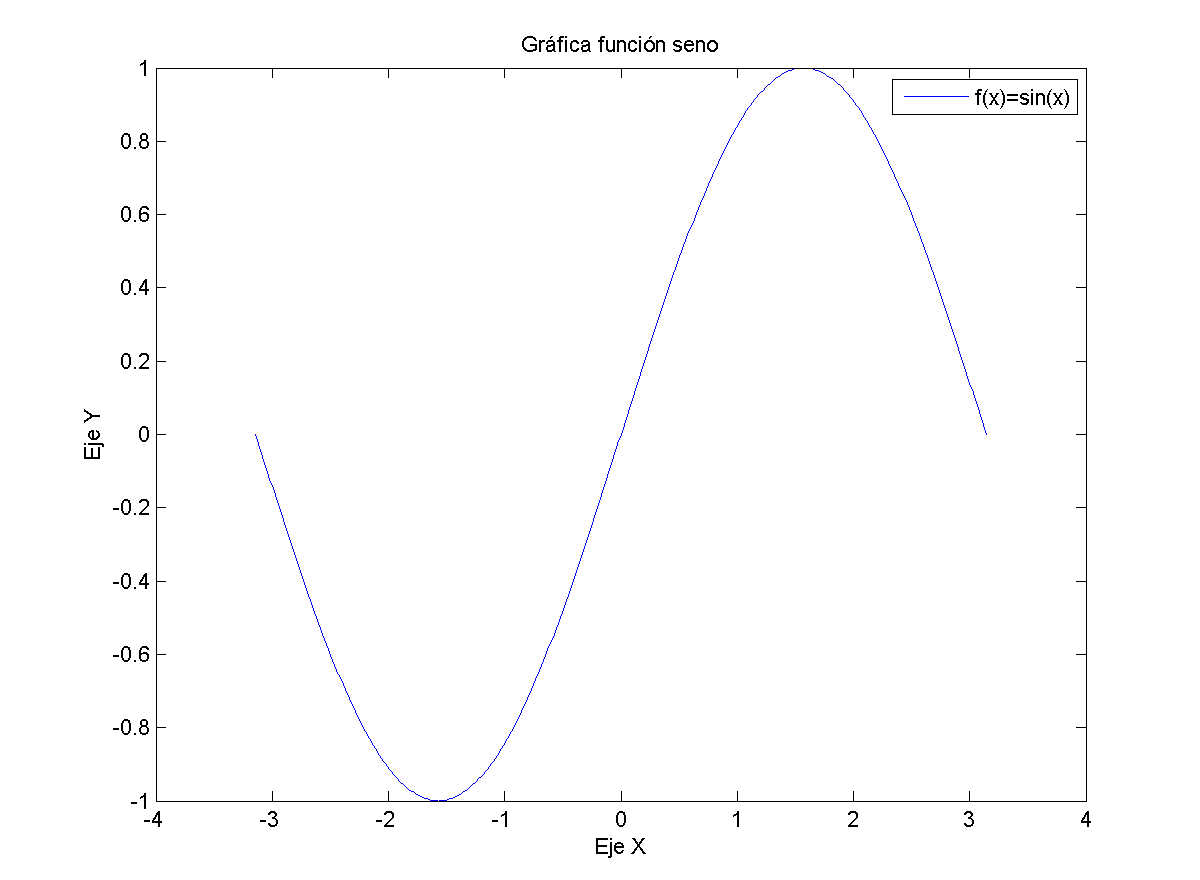
\includegraphics[scale=0.6]{src/ch4/img_4_4.png}
\captionof{figure}{Añadiendo etiquetas y título}
\end{center}

Las gráficas anteriores se han trazado utilizando el estilo por defecto que emplea MATLAB, 
es decir, una línea continua en color azul, pero  es posible modificar el color, grosor y 
el estilo de línea de las gráficas de modo que se ajuste a los requerimientos o a las 
exigencias visuales de cada individuo.

\subsubsection{Modificando el color de línea}

Para modificar el color de una gráfica basta con añadir como tercer argumento de la 
función plot uno de los modificadores de color que se indican en la siguiente tabla:

\begin{table}[h!]
\centering
{\rowcolors{1}{}{gray!20}
\begin{tabular}{p{4cm} p{4cm}}\hline
\rowcolor{LightBlue2} COLOR & MODIFICADOR \\
Rojo & \texttt{'r'} \\
Verde & \texttt{'g'} \\
Azul & \texttt{'b'} \\
Cyan & \texttt{'c'} \\
Magenta & \texttt{'m'} \\
Amarillo & \texttt{'y'} \\
Negro & \texttt{'k'} \\ 
Blanco & \texttt{'w'} \\
\end{tabular}
\caption{Modificadores de color}
\end{table}

La sintaxis de la función plot para una línea color verde sería:

\begin{verbatim}
	plot(x,y,'g');
\end{verbatim}

Además de los modificadores anteriores puede utilizarse un vector de tres elementos 
RGB para especificar el color, pero en este caso tiene que especificarse como argumento 
la propiedad que se modifica, es decir color, con lo cual la sintaxis bajo este método 
para trazar una línea color verde sería como sigue:

\begin{verbatim}
	plot(x,y,'color',[0 1 0]);
\end{verbatim}

\subsubsection{Configurar ejes (función axis)}

El comando / función axis permite hacer modificaciones a la apariencia y escala de los 
ejes en los cuales se trazan las gráficas. La sintaxis varía dependiendo de la 
característica a modificar.\\

\textit{Estableciendo los límites de una gráfica}\\

Para establecer los límites en los cuales se mostrará una gráfica puede introducir 
como argumento de la función axis un vector de 4 (gráficas en 2D) o 6 elementos 
(gráficas en 3D) con la sintaxis:

\begin{verbatim}
	axis([xmin xmax ymin ymax]); % Dos dimensiones
	axis([xmin xmax ymin ymax zmin zmax]); % Tres dimensiones
\end{verbatim}

Los elementos del vector deben ser de tipo double.\\

\textit{Ocultar o mostrar etiquetas, marcas, y ejes}\\

Si requiere ocultar los ejes, etiquetas, leyendas y demás marcas en las gráficas, de tal 
manera que sólo sea visible la línea trazada, utilice la función axis con el argumento 
\texttt{'off'}. Las siguientes líneas de código producen la imagen adjunta:

\begin{verbatim}
	x=linspace(-2*pi,2*pi,200);
	y=x.*cos(x);
	plot(x,y);
	axis off
\end{verbatim}

\begin{center}
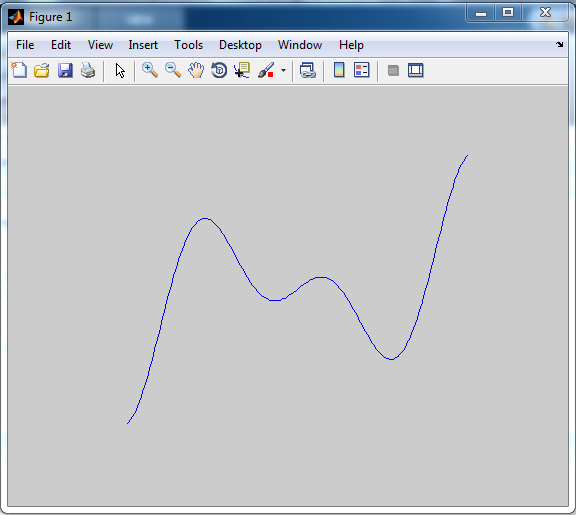
\includegraphics[scale=0.6]{src/ch4/img_4_5.png}
\captionof{figure}{Ocultando los ejes}
\end{center}

\textit{Escalado de ejes}\\

Además de permitir una configuración manual de los límites de ejes mediante la inserción 
de valores, es posible también establecer límites mediante modificadores que configuran 
los ejes y su apariencia de forma predeterminada. Los más comunes se enlistan y describen 
en la tabla siguiente.

\begin{table}[h!]
\centering
{\rowcolors{1}{}{gray!20}
\begin{tabular}{p{4cm} p{10cm}}\hline
\textbf{SINTAXIS} & \textbf{DESCRIPCIÓN} \\
\texttt{axis('equal')} & Ajusta el escalado de los ejes de tal modo que sean iguales en cada dirección. \\
\texttt{axis('square')} & Configura y ajusta la visualización de los ejes a un cuadrado o cubo (3D) \\
\texttt{axis('tight')} & Ajusta los ejes al rango de datos disponibles. \\
\end{tabular}
\caption{La función axis}
\end{table}

\subsubsection{Añadir anotaciones}

\subsection{Gráficas en coordenadas polares}

En el sistema de coordenadas polares cada punto del plano está definido por un ángulo y 
una distancia medidos respecto al eje polar y al polo, respectivamente. Generalmente para 
la notación de una ecuación polar se utilizan la letra griega $\theta$ para el ángulo 
y una r o $\rho$ para designar la distancia, siendo común la designación $r(\theta)$ para 
referir a una función en coordenadas polares.

Para graficar en coordenadas polares MATLAB dispone de la función polar cuya sintaxis es:

\begin{verbatim}
	polar(theta,rho);
\end{verbatim}

Ejemplo. Grafique la ecuación   (espiral)

\begin{verbatim}
	theta=0:pi/180:6*pi;
	r=theta;
	polar(theta,r);
\end{verbatim}

\begin{center}
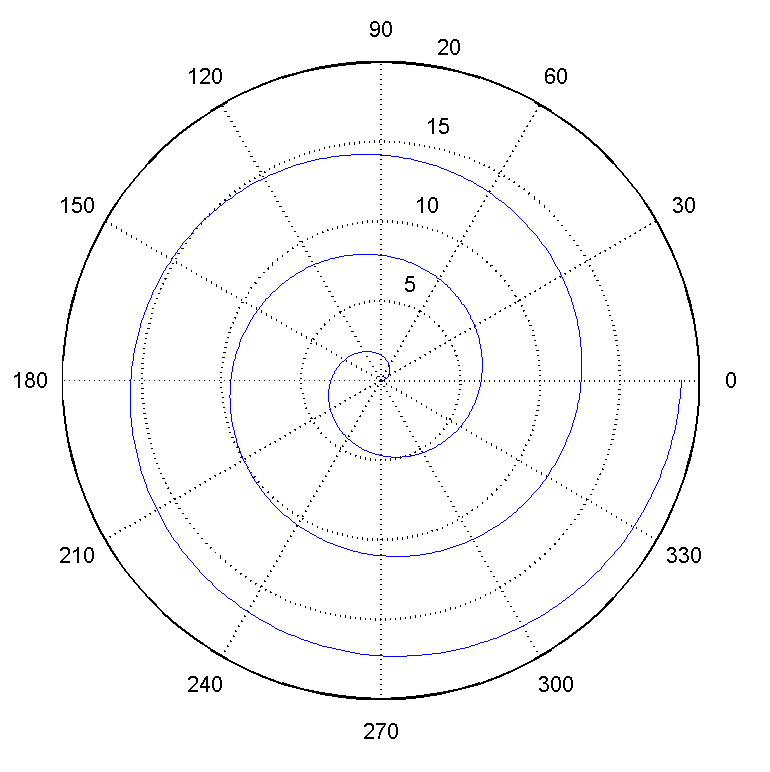
\includegraphics[scale=0.6]{src/ch4/img_4_6.png}
\captionof{figure}{Gráfica de una espiral en coordenadas polares}
\end{center}

Pese a que MATLAB cuenta con la función polar para facilitar el trazado de gráficas en 
coordenadas polares, es muy sencillo graficar estas utilizando la función plot con una 
conversión de coordenadas previa, por ejemplo, para la misma función anterior:

\begin{verbatim}
	theta=0:pi/180:6*pi;
	r=theta;
	x=r.*cos(theta); % Conversión de coordenadas 
	y=r.*sin(theta);
	plot(x,y);
\end{verbatim}

\section{Gráficas en tres dimensiones}

\subsection{Gráficas de superficies: una primera aproximación}

La representación gráfica de una función de dos variables $f(x,y)$ es una superficie 
trazada en un espacio tridimensional, resultante de la evaluación de la función en 
intervalos determinados para cada variable independiente.\\

A manera de ejemplo crearemos una matriz con los valores resultantes de la evaluación 
de la función en un punto específico; comenzaremos definiendo una función anónima de 
dos variables y enseguida utilizar ciclos for anidados para evaluar la función en 
cada punto. Véase el ejemplo mostrado a continuación:

\begin{verbatim}
	f=@(x,y) x.^2+y.^2;
	X=-5:0.2:5;
	Y=-5:0.2:5;
	for i=1:length(X)
	    for j=1:length(Y)
	        Z(i,j)=f(X(i),Y(j));
	    end
	end
	surf(Z);
\end{verbatim}

\begin{center}
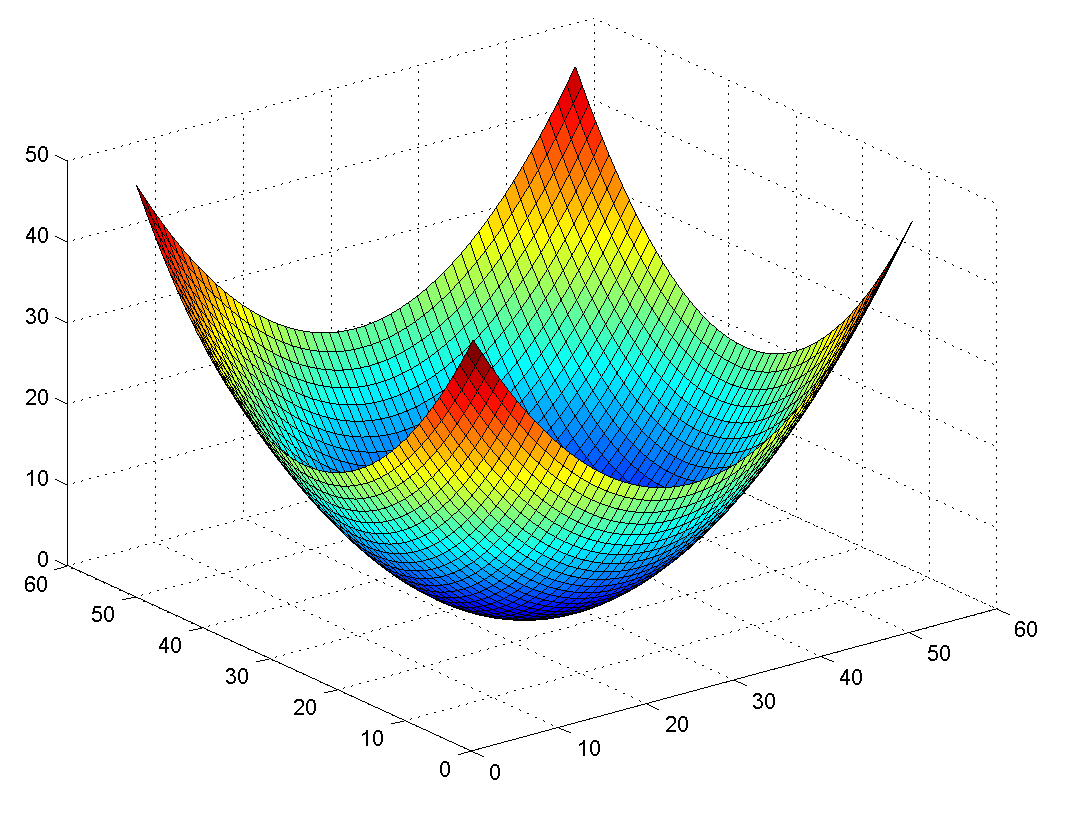
\includegraphics[scale=0.6]{src/ch4/img_4_7.png}
\end{center}

La función \texttt{surf} en el ejemplo anterior recibe como argumento de entrada una matriz bidimensional 
cuyos valores corresponden a cada punto evaluado. El código mostrado es funcional y muy entendible 
para un usuario que comienza en el mundo MATLAB, e incluso podría hacerse más "portable" o "reutilizable" 
si se definiese como una función, pero presenta ciertos inconvenientes: los ciclos for en MATLAB son 
generalmente conocidos por su lentitud, y más aún, en este caso se tienen dos ciclos for anidados. 
Debido a ello, MATLAB proporciona funciones que realizan la "tarea" de evaluar una función de dos 
variables en un rango definido mediante la implementación de rejillas bidimensionales (meshgrid), estas 
funciones se encuentran optimizadas mediante la técnica de vectorización y permiten una ejecución 
notablemente más veloz.

\subsection{Gráficas de superficies}

En el apartado anterior se ha visto como trazar superficies utilizando ciclos for anidados para crear 
la matriz que define los valores de la función de dos variables, pero ahora vamos a optimizar nuestro 
código utilizando la función \texttt{meshgrid} para definir el rango de valores a evaluar, la sintaxis 
de \texttt{meshgrid} es:

\begin{verbatim}
	>> [X,Y]=meshgrid(ix,iy);
\end{verbatim}

Donde X e Y son las matrices que definen el rango para las variables independiente y que se utilizarán 
para evaluar en una determinada función, ix e iy son vectores que definen el intervalo a evaluar de 
cada variable independiente. A continuación se muestra un ejemplo completo de cómo utilizar meshgrid 
en conjunto con surf para crear una gráfica de la función $f(x,y)=cos(x) sin(y)$:

\begin{verbatim}
	ix=0:0.2:10;
	iy=-5:0.2:5;
	[X,Y]=meshgrid(ix,iy);
	Z=cos(X).*sin(Y);
	surf(X,Y,Z);
\end{verbatim}

\begin{center}
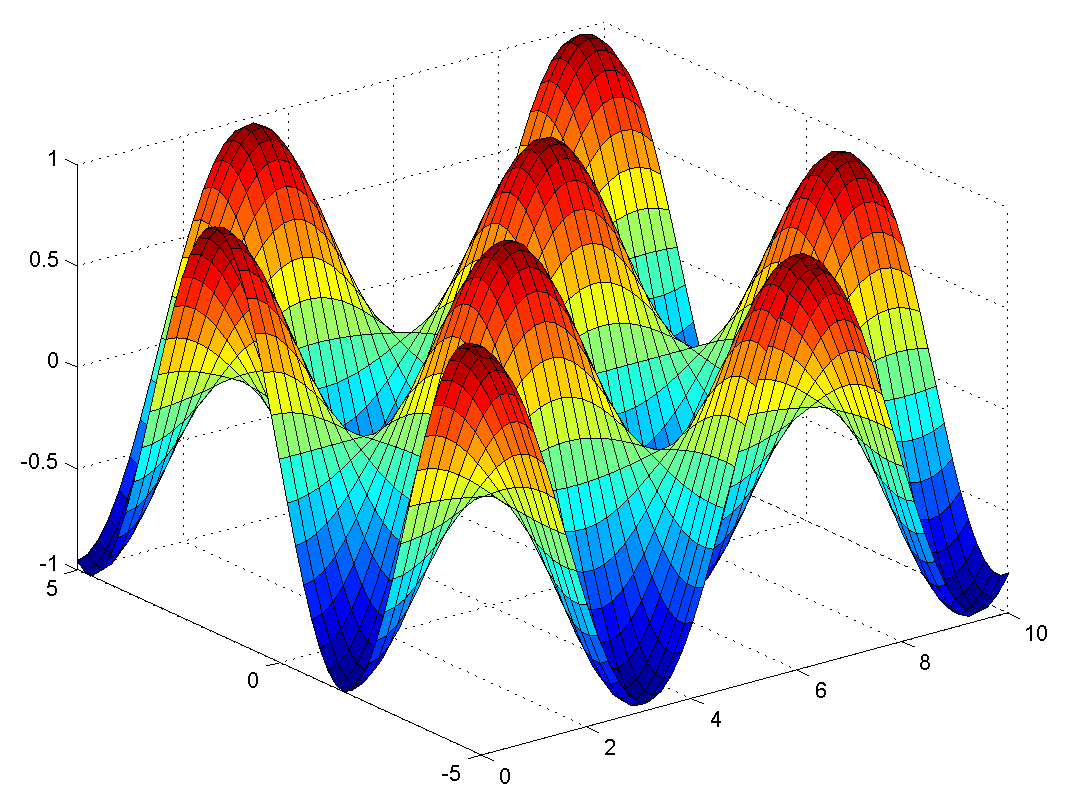
\includegraphics[scale=0.6]{src/ch4/img_4_8.png}
\end{center}

Note  que las operaciones de multiplicación o división deben estar vectorizadas, es decir, 
colocar un punto antes de cada operador correspondiente para indicar que se debe operar 
elemento a elemento. De lo contrario MATLAB devolverá un error o más grave aún: un resultado incorrecto.\\

Si ambos intervalos X e Y son iguales, puede proporcionar solo un argumento a la 
función meshgrid, es decir, es lo mismo tener esto:

\begin{verbatim}
	[X,Y]=meshgrid(1:10,1:10);
\end{verbatim}

que lo siguiente:

\begin{verbatim}
	[X,Y]=meshgrid(1:10);
\end{verbatim}

Claro que por cuestiones de comodidad sería preferible esta última, aunque quizá afecte 
un poco la legibilidad de un programa de mayores dimensiones, pero vamos, nada "catastrófico".

\subsection{Mapas de colores, sombreado e iluminación}

\subsubsection{Mapas de colores}

Un mapa de color es, en su definición más simplista, una matriz de m x 3 elementos 
cuyos valores se encuentran en el intervalo de 0 a 1, y donde cada fila representa 
un vector que especifica un color en el formato o modelo de color RGB. Pero, aquí 
la cuestión interesante es ¿para qué sirve un mapa de color?; así pues, un mapa de 
color no es más que un conjunto de colores que habrán de utilizarse para "pintar" 
una superficie de acuerdo a sus valores, pudo notar que en las superficies trazadas 
en los apartados anteriores se utiliza un color rojo para los valores más grandes y 
un color azul para los más pequeños, pasando por otras tonalidades para valores 
intermedios. Debe saber que esa "forma de colorear" la superficie está definida 
mediante un mapa de color por defecto, generalmente jet. Aparte de jet MATLAB 
cuenta con otros mapas de colores predefinidos que se muestran a continuación:

\begin{center}
\includegraphics[scale=1]{src/ch4/img_4_9.png}
\end{center}

Si teclea en MATLAB el nombre de cualquiera de los mapas de colores mostrados se devuelve 
una matriz de 64x3 elementos de tipo double, por ejemplo:

\begin{verbatim}
	>> map_color=hsv;
	>> whos map_color
	  Name            Size            Bytes  Class     Attributes

	  map_color      64x3              1536  double          
\end{verbatim}

Pero todo esto no tiene efecto sobre alguna superficie dibujada, para cambiar o configurar 
el mapa de color actual puede utilizar la función \texttt{colormap}, pasando un mapa de color como 
argumento, por ejemplo:

\begin{verbatim}
	[X,Y]=meshgrid(0:0.2:3*pi);
	Z=cos(X).*sin(Y);
	surf(X,Y,Z);
	colormap(hot);
\end{verbatim}

\begin{center}
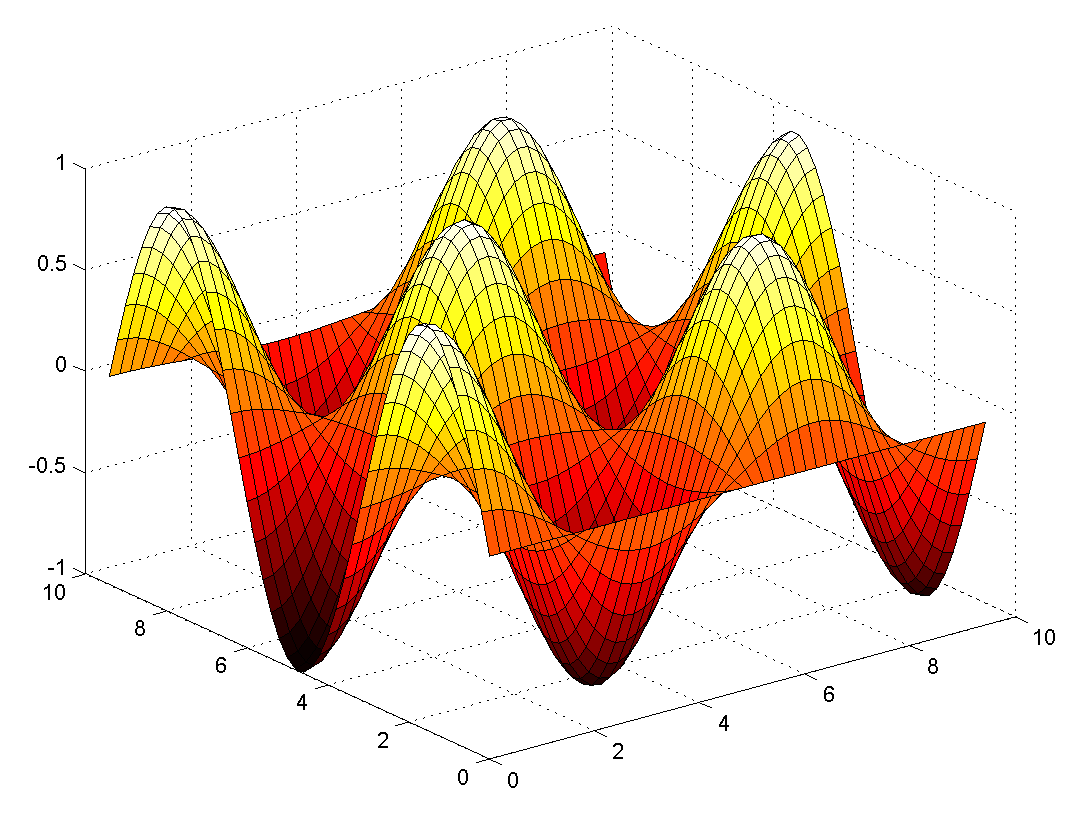
\includegraphics[scale=0.6]{src/ch4/img_4_10.png}
\end{center}

Interesante, sobre todo para quienes deseen darle a sus gráficos una mayor calidad 
estética o acorde a los datos que esté representando.\\

Si por alguna razón ninguno de los mapas de colores predefinidos le "convence", puede 
definir su propio mapa de color sin muchas complicaciones, para ello debe crear una 
matriz de m x 3 elementos donde cada fila contenga información acerca de un color en 
formato RGB, tomando en cuenta que el color ubicado en la primera fila será asignado 
al valor más pequeño y la última fila al mayor. Revise el siguiente ejemplo en el 
cual se define un mapa de color mediante cierta secuencia:

\begin{verbatim}
	Z=membrane;
	surf(Z);
	v=(1:10)'/10;
	cmap=[v flipud(v) flipud(v)];
	colormap(cmap);
\end{verbatim}

\begin{center}
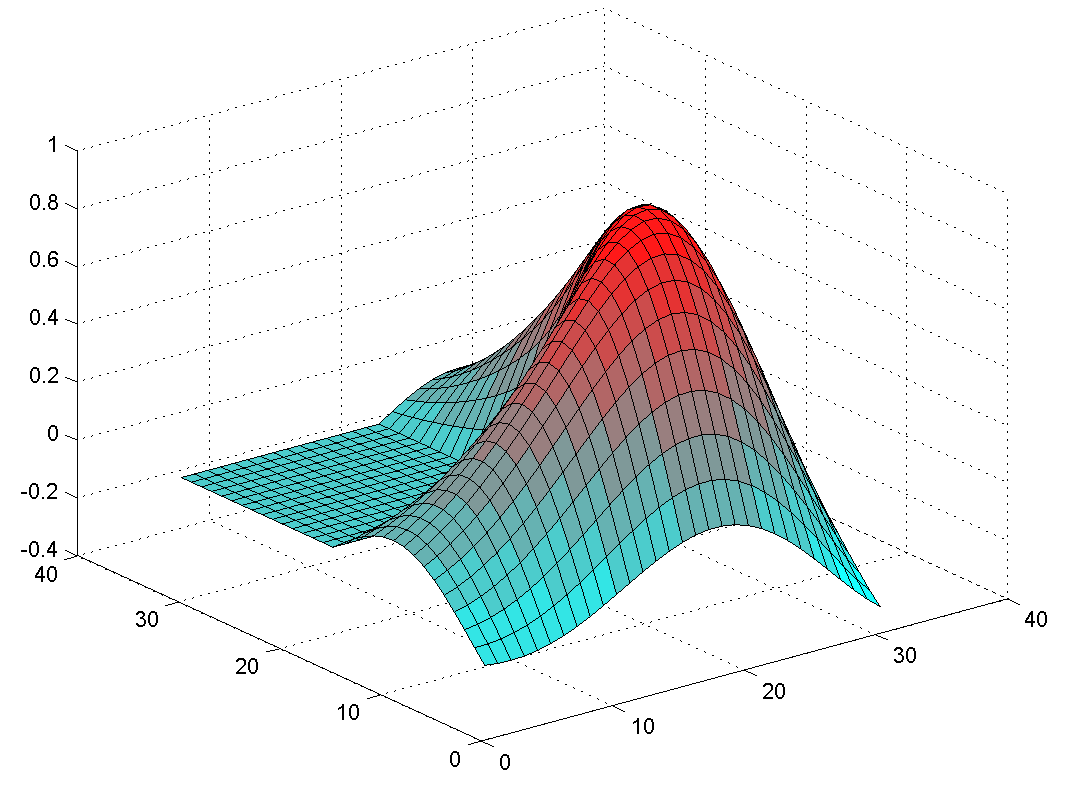
\includegraphics[scale=0.6]{src/ch4/img_4_11.png}
\end{center}

El resultado es una interesante variación de tonalidades ¿azul? a rojo. Por supuesto 
que  usted tiene todas las libertades para experimentar con diversas secuencias de 
colores y "adoptar" la que mejor le resulte.

\subsubsection{Sombreado}

Para efectos de esta sección, con sombreado se refiere a la forma en que MATLAB 
\textit{pinta} o \textit{rellena} los diversos componentes o parches (patch) que 
conforman una superficie.\\

En MATLAB existen tres tipos de sombreado que pueden controlarse mediante la función 
\texttt{shading}, los cuales son:

\begin{itemize}
\item faceted
\item flat
\item interp
\end{itemize}

El tipo \texttt{faceted} es el sombreado por defecto, y se caracteriza por pintar cada 
parche de la superficie utilizando un color sólido de relleno y un borde en color negro.\\

El tipo \texttt{flat} funciona de manera similar al anterior, con la diferencia que el borde 
adquiere el mismo color que el interior del parche.\\

Y el tipo \texttt{interp} se vale de una interpolación de la matriz que define el mapa de 
color actual para pintar de forma cuasi-continua y con variaciones menos "bruscas" a 
cada parche, de hecho con este tipo de sombreado es imposible distinguir cada pieza 
que compone la superficie.\\

La función \texttt{shading} sólo necesita como argumento el tipo de sombreado, por ejemplo:

\begin{verbatim}
	>> shading('flat')
\end{verbatim}

Incluso acepta la notación de comandos, es decir, la siguiente forma también es válida:

\begin{verbatim}
	>> shading flat
\end{verbatim}

\subsubsection{Iluminación}

\section{Animaciones}

\subsection{Mi primera animación, una introducción}

Quizá parezca un poco lógico que para realizar una animación debe hacerse uso de bucles 
(for o while), dado que estos permiten variaciones durante el tiempo que se ejecutan. 
Tómese como ejemplo el siguiente código:

\begin{verbatim}
	x=0:0.01:10;
	for i=1:10
	    plot(x,sin(x+i));
	end
\end{verbatim}

Si ejecuta el código anterior comprobará que únicamente le será visible la última 
gráfica que corresponde al valor de i=10, es decir de la función   ; las demás gráficas 
también se muestran pero durante un lapso de tiempo demasiado breve como para percibirlo. 
Para ralentizar la ejecución del bucle for puede utilizarse la función pause que permite 
detener la ejecución de un programa durante un periodo de tiempo especificado en segundos; 
modificando el código anterior podemos “mejorar” nuestra animación.

\begin{verbatim}
	x=0:0.01:10;
	for i=1:10
	    plot(x,sin(x+i));
	    pause(0.1);
	end
\end{verbatim}

Ahora es posible visualizar el cambio efectuado en cada ejecución del ciclo for, siendo en 
este caso el desplazamiento de la función seno; en cada  ciclo MATLAB detiene durante 0.1 
segundos la ejecución, lo que permite al usuario visualizar cada una de las gráficas como 
un continuo animado.\\

Una vez conocido lo anterior, podemos añadir variaciones no solamente en la forma, sino 
también en el color de la gráfica utilizando vectores formados por valores aleatorios en 
cada secuencia, por ejemplo una modificación de ese tipo sería:

\begin{verbatim}
	x=0:0.01:10;
	for i=1:10
	    plot(x,sin(x+i),'linewidth',2,'color',rand(1,3));
	    set(gca,'color',rand(1,3));
	    pause(0.1);
	end
\end{verbatim}

Verifique los resultados de la animación. Claro que las modificaciones que pueden hacerse 
dependen de la imaginación, creatividad o de la necesidad de cada usuario. En la siguiente 
imagen se muestra la secuencia correspondiente a la animación.

\begin{center}
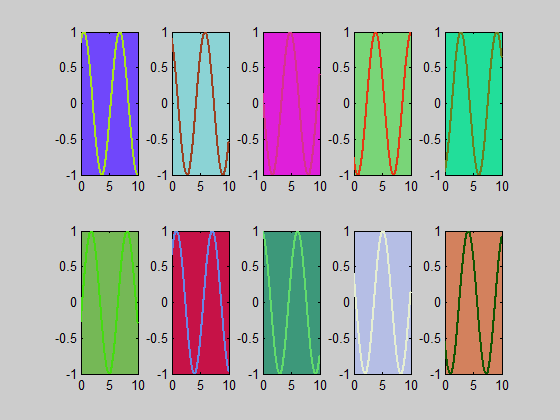
\includegraphics[scale=0.6]{src/ch4/img_4_12.png}
\end{center}